\setlength{\tabcolsep}{.1cm}
\begin{figure*}[!t]
\begin{tabular}{c c}
    \centering
% Suggestion 1: Always specify either height or weight
% Suggestion 2: Make sure the aspect ratio when exported matches the intended ratio in the paper here
    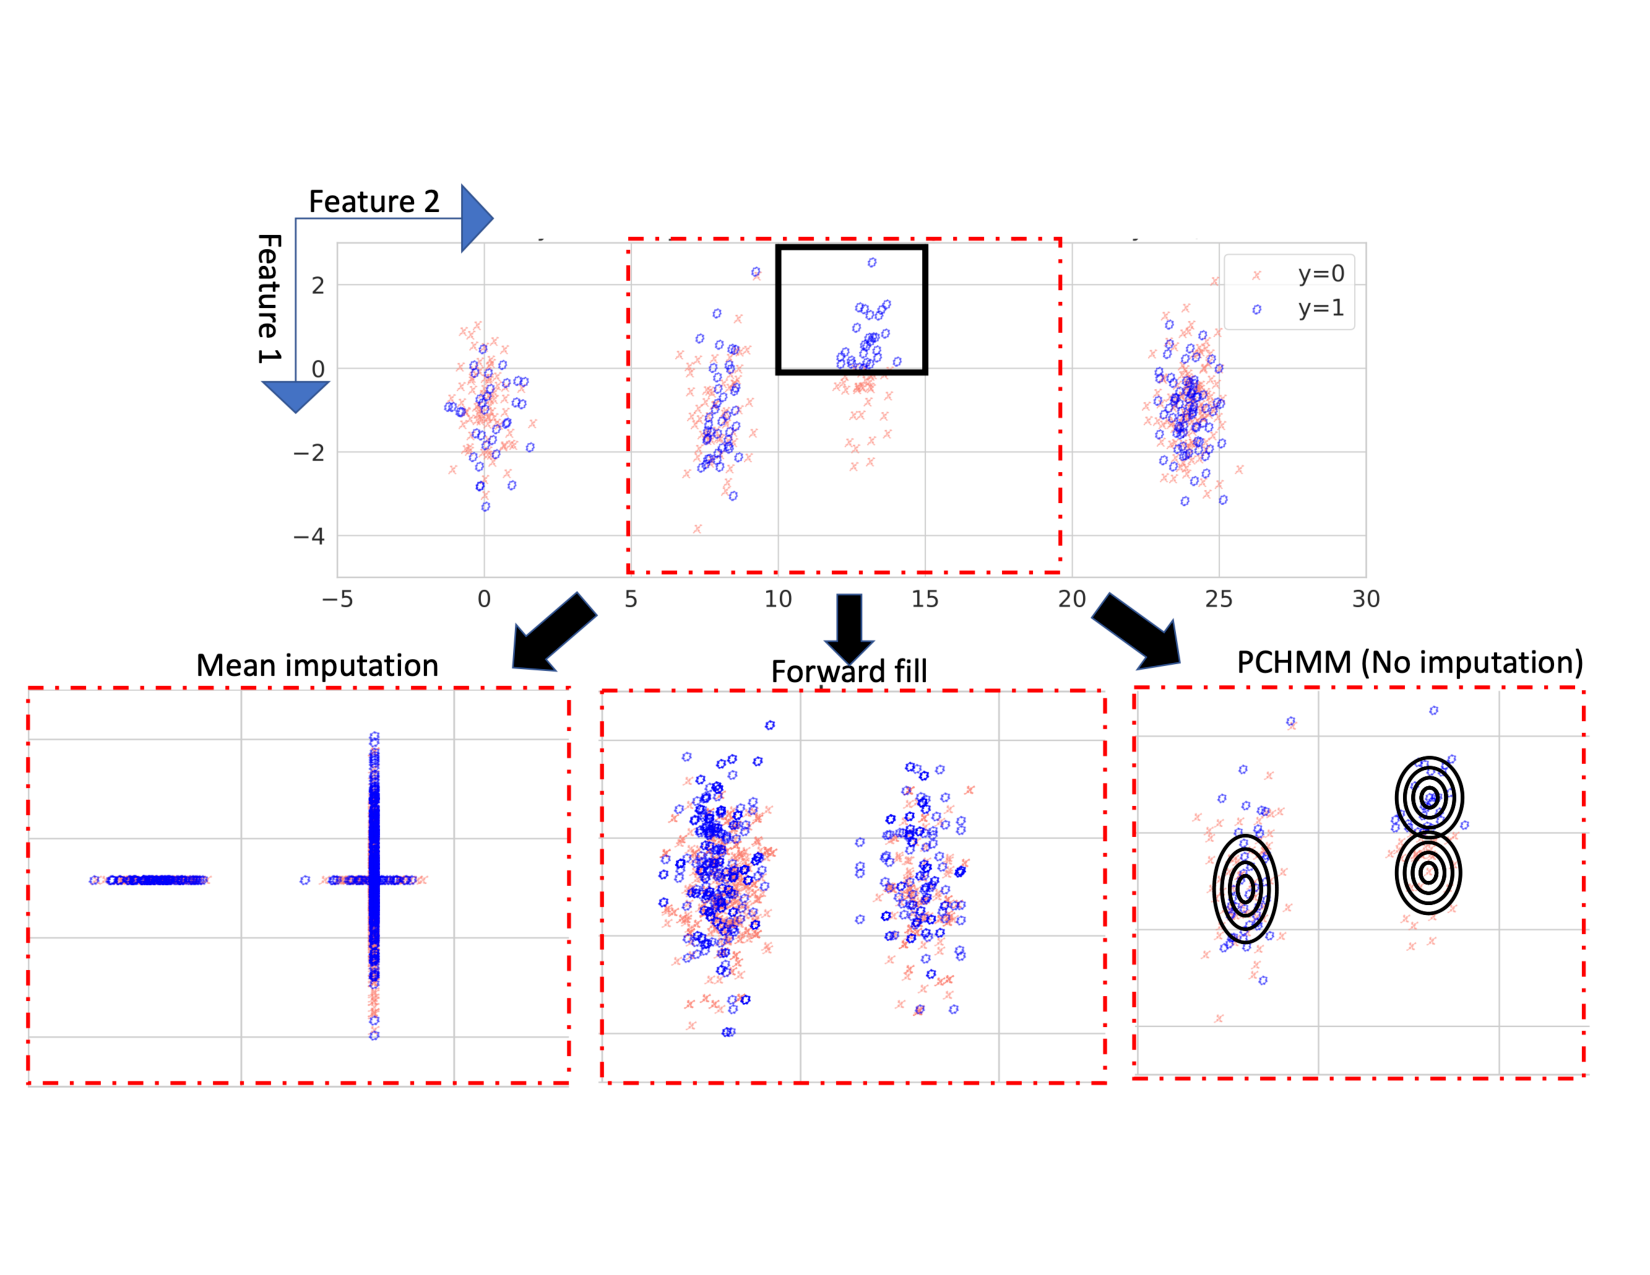
\includegraphics[width=0.57\textwidth]{content/chapters/semi_supervised_pchmm_missing_data/images/toy_data_fig.pdf}
    &
    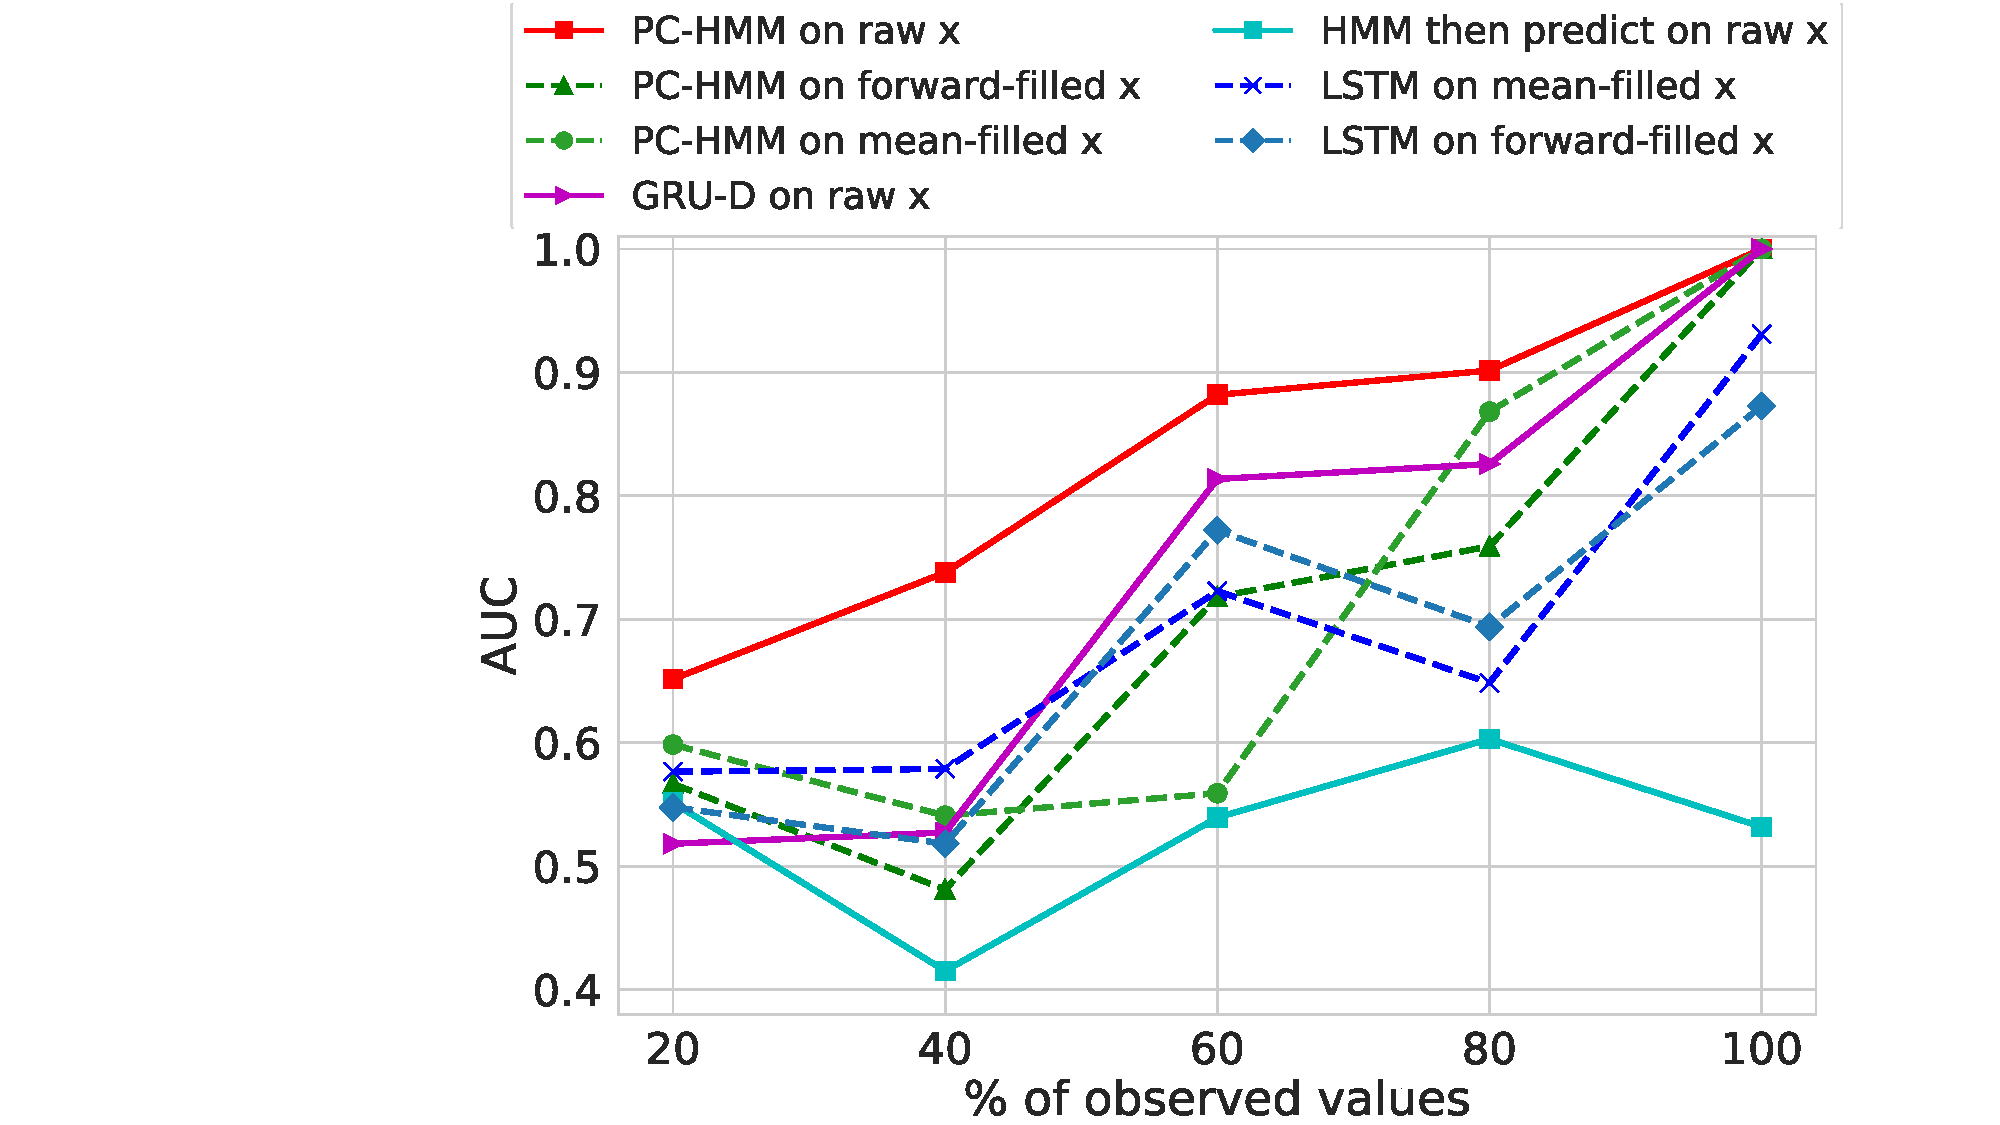
\includegraphics[width=0.43\textwidth]{content/chapters/semi_supervised_pchmm_missing_data/images/toy_data_perf_fig.pdf}
\end{tabular}
\caption[Demonstration of proposed PC-HMM on an “easy” binary classifier
task where naive imputation fails]{Demonstration of proposed PC-HMM on an ``easy'' binary classifier task where naive imputation fails.
\textbf{\emph{Top left:}} Visualization of all observed 2D features from 350 sequences (x-axis: feature 1 value, y-axis: feature 2), colored by labels and collapsed over time.
Each sequence ($T{=}8$) comes from a Markov model that generates features from the 4 clusters shown in this 2D feature space.
A sequence's class label depends on if \emph{any observation} lands in the black box (yes means $y=1$, no means $y=0$). 
Without missingness, the two classes are clearly separable: compare black box to region below it.
\textbf{\emph{Bottom left:}} We sample features as missing with 40\% probability i.i.d. across timesteps and features. We then apply mean-filling or forward-filling: each panel shows 2D values \emph{after} imputation.
Either strategy clearly destroys class separability. 
Our PC-HMM does not need imputation, and even at 40\% missingness can learn to separate the black box from the region below it with separate Gaussian emission densities (black elipsoids).
\textbf{\emph{Right:}} AUROC vs. percentage of feature values observed. Across every tested percentage, our PC-HMM with compact state space (only 6 states, 80 total parameters) can outperform GRU-D or LSTM models even with many more parameters. 
}%endcaption
\label{fig:toy_pchmm}
\end{figure*}